%   MSc Business Analytics Dissertation
%   Format based on skeleton template provided as part of module MIS40750
%
%   Title:     Optimising the design of buffer preparation in bioprocessing
%              facilities
%   Author:    Sean Tully
%
%   Chapter 5: Results
%
%   Change Control:
%   When     Who   Ver  What
%   -------  ----  ---  --------------------------------------------------------
%   06Jun16  ST    0.1  Begun 
%

\chapter{Results}\label{C.results}

\begin{quote}
Bosh! Stephen said rudely.
A man of genius makes no mistakes.
His errors are volitional and are the portals of discovery.

\hspace{2cm}--- James Joyce, \emph{Ulysses}
\end{quote}

\section{Output Data}\label{S.outputdata}
The primary aim is to generate a list of the required preparation volumes.
For the random example used in this chapter, solution of the model yields
the results in \hyperref[tbl.reqvessels]{Table \ref*{tbl.reqvessels}}.

\begin{table}[h!]
    \centering
    \caption{Required preparation vessels for random example}
    \label{tbl.reqvessels}
    \begin{tabular}{r}
        vessel size\\ \hline
        \SI{2000}{\litre}\\
        \SI{8000}{\litre}\\
        \SI{25000}{\litre}\\
        \SI{30000}{\litre}\\
    \end{tabular}
\end{table}

While \hyperref[tbl.reqvessels]{Table \ref*{tbl.reqvessels}} gives the
essential information allowing the buffer preparation area to be sized and
costed, it may be more instructive to return a matrix showing where each buffer
is to be prepared.
Indeed, the presentation of such a minimal manifestation of results is
unlikely to convince a client of the feasibility of the solution.

\begin{table}[t]
    \centering
    \caption{Buffer / vessel matrix for random example}
    \label{tbl.bvmatrix}
    \begin{tabular}{l | c | c | c | c }
        & \SI{2000}{\litre} & \SI{8000}{\litre} & \SI{25000}{\litre} &
        \SI{30000}{\litre}\\ \hline
        Buffer \#1  & & & $\bullet$ & \\
        Buffer \#2  & & $\bullet$ & & \\
        Buffer \#3  & & $\bullet$ & & \\
        Buffer \#4  & & $\bullet$ & & \\
        Buffer \#5  & $\bullet$ & & & \\
        Buffer \#6  & & & $\bullet$ & \\
        Buffer \#7  & & & & $\bullet$ \\
        Buffer \#8  & & & & $\bullet$ \\
        Buffer \#9  & & & & $\bullet$ \\
        Buffer \#10 & & $\bullet$ & & \\
        Buffer \#11 & & & $\bullet$ & \\
        Buffer \#12 & & & $\bullet$ & \\
    \end{tabular}
\end{table}

\hyperref[tbl.bvmatrix]{Table \ref*{tbl.bvmatrix}} shows \emph{one possible}
vessel assignment for the random example.
Note that the existence of more than one feasible version of 
\hyperref[tbl.reqvessels]{Table \ref*{tbl.reqvessels}} is unlikely for a given
data-set, especially if vessel cost scales non-linearly with vessel volumes.
On the other hand, many feasible versions of
\hyperref[tbl.bvmatrix]{Table \ref*{tbl.bvmatrix}} may exist; e.g.\ it may be
possible to switch the vessels in which buffers are prepared and still end up
with the same optimal vessel selection.
This phenomenon is dealt with in more detail in 
\hyperref[S.secondary]{Section \ref*{S.secondary}}.

While \hyperref[tbl.bvmatrix]{Table \ref*{tbl.bvmatrix}} does give more
information than \hyperref[tbl.reqvessels]{Table \ref*{tbl.reqvessels}},
it still doesn't visibly confirm to the reader that the solution is feasible.
An \emph{equipment time utilisation} plot provides a clear visual illustration
of a solution and displays a feasible schedule.
The explanatory plot in 
\hyperref[fig.explanatory]{Figure \ref*{fig.explanatory}} is an example of an
equipment time utilisation plot.

An equipment time utilisation plot for the random example data detailed in
\hyperref[C.data]{Chapter \ref*{C.data}} is shown in
\hyperref[fig.etu1]{Figure \ref*{fig.etu1}}.
\begin{figure}
    \centering
    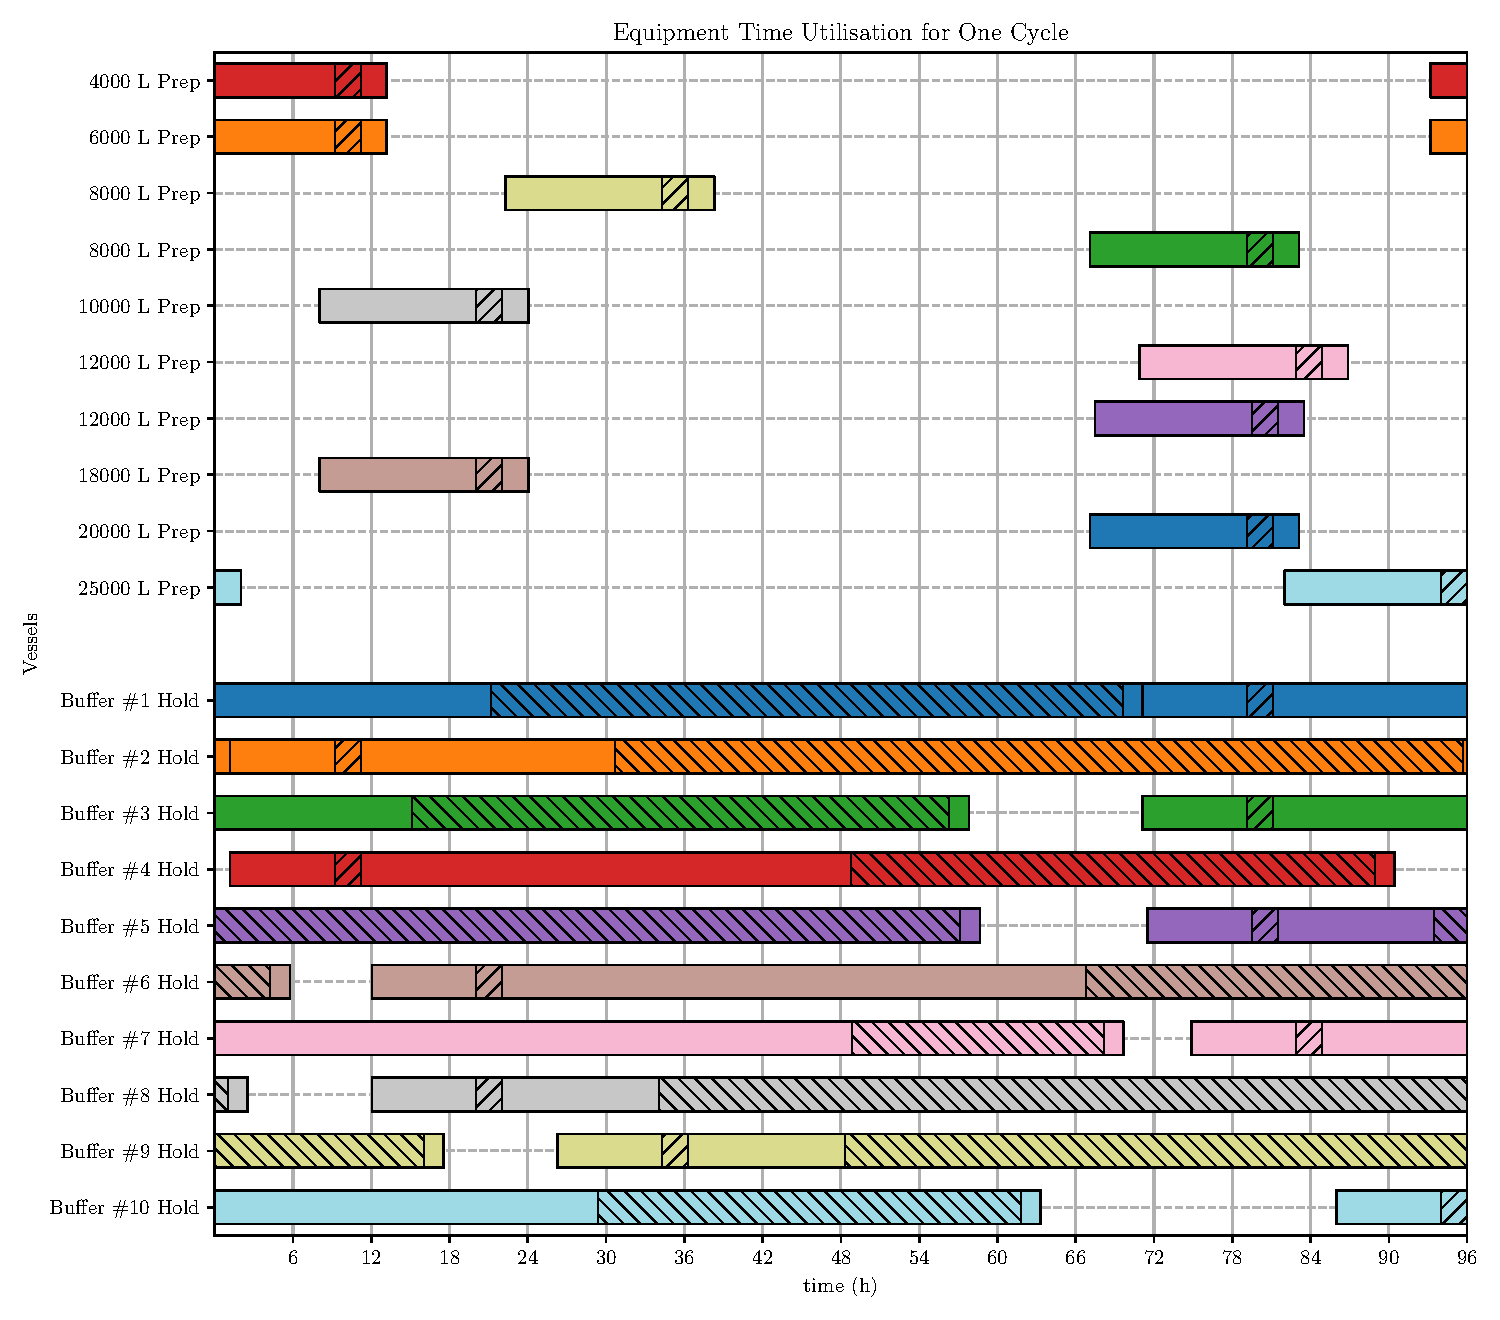
\includegraphics[width=\linewidth]{./figures/plot1.pdf}
    \caption{Equipment time utilisation for random example}
    \label{fig.etu1}
\end{figure}
Each horizontal dotted line represents a piece of equipment (preparation or
hold vessels in this case).
The presence of a bar on a dotted line indicates that the respective piece of
equipment is in use.  
The hatched bars indicate transfers, as per the legend.

Transfer from a buffer hold vessel to the production process is shown as a
contiguous bar in the hold vessel, representing the
period from the start of the first use to the end of the last use of the buffer
in a given batch, although the demand from the production process may be
discontinuous.

The bars are coloured by buffer. Since the buffer hold vessels are dedicated
to particular buffers, and are named according to the buffers they contain,
the buffer hold entries serve as a legend for the colour scheme.

Note that the time window shown in \hyperref[fig.etu1]{Figure \ref*{fig.etu1}}
displays a single cycle at steady-state; the next cycle and the previous cycle
would be identical.
The offset of the single-cycle window is somewhat arbitrary; the
visible window can be thought of as a cylinder that has been cut at right a
angles to its ends and flattened out.

It should be noted also that \hyperref[fig.etu1]{Figure \ref*{fig.etu1}}
does not highlight the batches to which the procedures belong.
The entire downstream process may take more than one cycle to complete, so the
window visible in the plot could be showing buffer preparation and hold
procedures from several successive batches.

The visual output of an equipment time utilisation plot provides a useful
method for validating results.
As the model detailed in 
\hyperref[C.methodology]{Chapter \ref*{C.methodology}} was being developed,
such plots were a useful way of highlighting logical flaws or bugs in the code.
With the finished model, such plots are a useful tool for convincing
colleagues and clients that a proposed vessel selection is indeed feasible.

\section{Solution Duration}\label{S.soltime}
\subsection{Variation of Problem Size}\label{SS.buffcount}
Using the parameters data set given in 
\hyperref[tbl.parameters]{Table \ref*{tbl.parameters}} and the vessels data set
given in \hyperref[tbl.vessel]{Table \ref*{tbl.vessel}}, the time taken for
the CPLEX solver to reach a feasible solution was evaluated for a range of 
randomly-generated buffer data sets of different sizes.

The runs were carried out on a computer with \SI{16}{\giga\byte} of RAM and an
Intel 3770K processor (four physical cores; eight virtual cores, running at
\SIrange{3.5}{3.9}{\GHz}).
The operating system was Arch Linux 64 bit (rolling release).
It was note that the CPLEX solver uses multi-threading effectively, as all
eight virtual cores were running at \SI{100}{\%} fairly consistently during the
runs (the usage tended to dip slightly at the start and end of each run).
RAM usage during the runs was below \SI{1}{\giga\byte}, so memory shortage was
not a factor in the solution durations.

\begin{figure}
    \label{fig.timing}
    \centering
    \includegraphics[width=\linewidth]{./figures/timing.pdf}
    \caption{Solution time as a function of buffer count}
\end{figure}

For a set of problem sizes (i.e.\ values of $N$), 100 random data sets
were generated for each problem size and the solution durations were recorded.
A box plot of the durations is shown in 
\hyperref[fig.timing]{Figure \ref*{fig.timing}}.
A total of \num{1000} runs were performed to generate
\hyperref[fig.timing]{Figure \ref*{fig.timing}} and for each run, an optimal
solution was found.
Note that there are several slow outliers for each problem size.
In the case of $N=20$, the highest outlier is approximately two
orders of magnitude greater than the mean duration, indicating a high degree
of variability.

Such variability in solution duration is not uncommon in MILP problems.
Methods for solving problems with binary variables necessarily involve some
searching through large binary trees, where search time can vary greatly
depending on the location of the optimum result and the search strategy.

\subsection{Comparison of Solvers}\label{SS.solvers}
A similar analysis to that carried out in
\hyperref[SS.buffcount]{Section \ref*{SS.buffcount}} was attempted with the
Cbc and GLPK solvers.
The results are shown in \hyperref[fig.timings]{Figure \ref*{fig.timings}}.
Each point represents the mean duration of 100 runs of a particular problem
size with a particular solver.

Both Cbc and GLPK were found to be considerably slower than CPLEX.

The GLPK solver is only capable of running single-threaded so cannot take
advantage of a multi-threaded processor.
It was the fastest at solving the trivial two-buffer problem, but showed the
steepest rate of solution time increase with increasing number of buffers.
At a size of $N=8$, GLPK showed massive variation in solution time, with
solutions ranging from less than 10 seconds to over 8 hours.  As a result,
only data points for $N=6$ and below are shown for GLPK.

The Cbc solver had better performance but had reliability issues; on three
random runs out of 100, with a problem size of $N=10$, Cbc was taking several
orders of magnitude longer than the mean to obtain a solution, so those runs
were halted.
While the CPLEX and GLPK solvers were called with no arguments, the
\texttt{threads=8} argument was passed to the Cbc solver to get it to use all
virtual cores on the computer (CPLEX uses all virtual cores by default and GLPK
only operates as a single thread).

CPLEX proved robust over the range $2 \le N \le 20$.

\begin{figure}
    \label{fig.timings}
    \centering
    \includegraphics[width=\linewidth]{./figures/timings.pdf}
    \caption{Solution time as a function of buffer count}
\end{figure}

Note that the data in \hyperref[fig.timings]{Figure \ref*{fig.timings}}
indicate that solution time is exponential in $N$, which is to be expected for
an \textbf{NP}-hard optimisation problem.

\subsection{Real-World Data}\label{SS.realworld}
The model was applied to (obfuscated) data from two real-world data sources.
In both cases, CPLEX found feasible solutions in under one minute.
The data and results for both real-world examples are recorded in an appendix
to this report.

